% COMP534 Assessment 3 — Chunking / Shallow Parsing
% Two-column, ≤1200 words, rubric-aligned
\documentclass[10pt,a4paper,twocolumn]{article}
\usepackage[margin=1.7cm]{geometry}
\usepackage{times}
\usepackage{latexsym}
\usepackage{amsmath,amssymb}
\usepackage{graphicx}
\usepackage{booktabs}
\usepackage{microtype}
\usepackage{hyperref}
\usepackage{xcolor}
\usepackage{enumitem}
\usepackage[numbers,compress,sort&compress]{natbib}
\usepackage{caption}
\usepackage{float}

% Formatting tweaks
\setlength{\bibsep}{1pt}
\setlength{\parskip}{1pt}
\setlength{\parindent}{0.9em}
\setlength{\columnsep}{18pt}
\captionsetup{font=footnotesize,labelfont=bf,skip=2pt}
\hypersetup{colorlinks=true,linkcolor=blue,citecolor=blue,urlcolor=blue}

% --- AUTHOR DATA ---
\title{\textbf{Neural Chunking: Comparative Study of RNN and Transformer Architectures}}
\author{Ainur Smailova, Nattanan Sottivorakun, Laura Valentina Sierra Peña, Saif Ur Rehman}
\date{}

\begin{document}

\twocolumn[{%
  \centering
  {\Large\bfseries Neural Chunking: Comparative Study of RNN and Transformer Architectures}\\[4pt]
  {\small COMP534 Assessment 3}\\[8pt]
  {\large Ainur Smailova, Nattanan Sottivorakun, Laura Valentina Sierra Peña, Saif Ur Rehman}\\[20pt]
}]

% ─────────────────────────────────────────────────────────────────────────────
\section*{Introduction}
\label{sec:intro}

Chunking (shallow parsing) labels every token with a BIO~\citep{Ramshaw1995,Sang1999}
tag identifying phrase boundaries and types. Using a corpus of 8{,}919 sentences
with 17 BIO labels, we compare six neural architectures spanning the recurrent
and self-attentive families, with structured (CRF) and softmax decoders.
The implementation uses only \texttt{nn.Linear}/\texttt{nn.Parameter} for the
Transformer and a hand-written linear-chain CRF.

% ─────────────────────────────────────────────────────────────────────────────
\section*{Data Management}
\label{sec:data}

\subsection*{Experimental Protocol}
We adopt a \emph{sentence-level} random 70/15/15 train/val/test split with
seed~42. Splitting at sentence granularity prevents leakage of recurrent
context across folds; token-level splitting would assign correlated tokens to
different sets. The validation set is used for model selection and early
stopping; the test set is held out and accessed exactly once. To strengthen
the generalisation estimate we additionally run \emph{5-fold cross-validation}
on the (train\,$\cup$\,val) pool for the best architecture, keeping the test
set sealed — the standard \emph{outer holdout + inner CV} protocol.

\subsection*{Dataloader and Preprocessing}
The corpus parser reads two-column word/tag rows, treating blank lines as
sentence delimiters; we recover 8{,}919 sentences (211{,}243 tokens). The
\emph{vocabulary is built on training data only} with min-frequency~$=2$,
yielding $|V|=7{,}755$; tokens below threshold map to \texttt{<UNK>}, giving an
8.95\% test-set OOV rate. We reserve $\texttt{<PAD>}=0$ for masking. Tags map
to integer ids; PAD positions use label $-100$ so PyTorch's
\texttt{CrossEntropyLoss(ignore\_index=-100)} excludes them from gradients.
Each batch uses \emph{dynamic padding} via a custom \texttt{collate\_fn}: tokens
are padded to the longest sequence in the batch, with explicit boolean masks
\texttt{(mask = ids != PAD)} threaded through every encoder, including
\texttt{pack\_padded\_sequence} for RNNs and key-padding masks in MHSA. The
class distribution is severely skewed (\texttt{I-NP}/\texttt{B-NP} together
$\approx39\%$ of tokens; \texttt{B-INTJ}/\texttt{B-CONJP} occur ${<}20$ times),
motivating macro-F1 and Cohen's~$\kappa$~\citep{Cohen1960} in the Evaluate Models section.

% ─────────────────────────────────────────────────────────────────────────────
\section*{Neural Networks}
\label{sec:nn}

\subsection*{Architectures}
All six models share a PAD-aware learned embedding \begin{itemize}
    \item \textbf{BiLSTM} \citep{Hochreiter1997} — 1-layer bidirectional LSTM with
    packed sequences; classifier $\mathbf{W}\!\in\!\mathbb{R}^{2H\times T}$.
    The simple RNN baseline.
    
    \item \textbf{DeepBiLSTM} \citep{Ma2016} — 2 stacked BiLSTM layers with inter-layer
    dropout, encouraging hierarchical representations: lower layer captures local
    boundary cues, upper integrates phrase-level context.
    
    \item \textbf{BiLSTM+CRF} \citep{Huang2015,Lample2016} — BiLSTM emissions feeding a
    \emph{manual} linear-chain CRF~\citep{Lafferty2001}; adds a $T{\times}T$
    transition matrix plus start/end vectors; trained by maximising the path
    log-likelihood
    $\mathcal{L}=-(\,e(y)-\log Z(\mathbf{x})\,)$ where $Z$ is the
    forward-algorithm partition function; decoded with Viterbi.
    
    \item \textbf{Transformer} \citep{Vaswani2017} — pre-norm encoder
    $\mathbf{x}\!\leftarrow\!\mathbf{x}+\text{Drop}(\text{MHSA}(\text{LN}(\mathbf{x})))$
    chosen for early-training stability~\citep{Xiong2020}; sinusoidal positional
    encoding; attention uses key-padding masks. Built from
    \texttt{nn.Linear}/\texttt{nn.Parameter} only.
    
    \item \textbf{Transformer+CRF} — same encoder, structured decoder; allows a
    decoder-only ablation against the plain Transformer.
    
    \item \textbf{TF(learned-PE)} — replaces sinusoidal with a trainable
    \texttt{nn.Embedding} over absolute positions; the PE-type ablation.
\end{itemize}

\subsection*{Training Components}
\begin{itemize}
    \item Loss: \texttt{CrossEntropyLoss} ignoring PAD for softmax models; CRF
    negative-log-likelihood for structured ones. 
    
    \item Optimiser: AdamW
    ($\beta\!=\!(0.9,0.999)$, $\lambda_{\text{wd}}\!=\!10^{-5}$); decoupled
    weight decay avoids the $L_2$ regularisation inconsistency of plain
    Adam~\citep{Loshchilov2019}. 
    
    \item Scheduler: ReduceLROnPlateau on val macro-F1
    (factor 0.5, patience 1). 
    
    \item Gradient norm clipped at 5.0 (RNN) and 1.0 (Transformer) — following \citet{Vaswani2017} for from-scratch attention training.
    
    \item Early stopping on val macro-F1 (patience 3). 
    
    \item Dropout 0.3 (RNN) / 0.1 (Transformer). 
    
    \item Epochs: 12 softmax / 10 CRF (CRF is $\sim5{\times}$ slower
    per step due to $O(LT^2)$ forward).
\end{itemize}

\begin{table}[t]\centering\footnotesize
\caption{Validation comparison (sorted by chunk-F1).
BIO~Valid: \% sequences with no illegal BIO transitions;
CRF decoders suppress illegal transitions via learned penalties
(BiLSTM+CRF: 97.0\%), softmax models have no such constraint (BiLSTM: 80.6\%).}
\label{tab:val}
\setlength{\tabcolsep}{3pt}
\begin{tabular}{@{}lrrrr@{}}
\toprule
Model & Params & ChF1 & MacF1 & BIO \\
\midrule
\textbf{DeepBiLSTM} & 3.37M & \textbf{0.892} & \textbf{0.736} & 88.0\% \\
BiLSTM+CRF  & 1.79M & 0.883 & 0.704 & \textbf{97.0\%} \\
BiLSTM      & 1.79M & 0.874 & 0.703 & 80.6\% \\
Trans.+CRF  & 1.26M & 0.811 & 0.510 & 71.2\% \\
TF(lrn-PE)  & 1.29M & 0.717 & 0.446 & 12.0\% \\
Transformer & 1.26M & 0.704 & 0.464 & 13.5\% \\
\bottomrule
\end{tabular}
\end{table}

\begin{figure}[t]
\centering
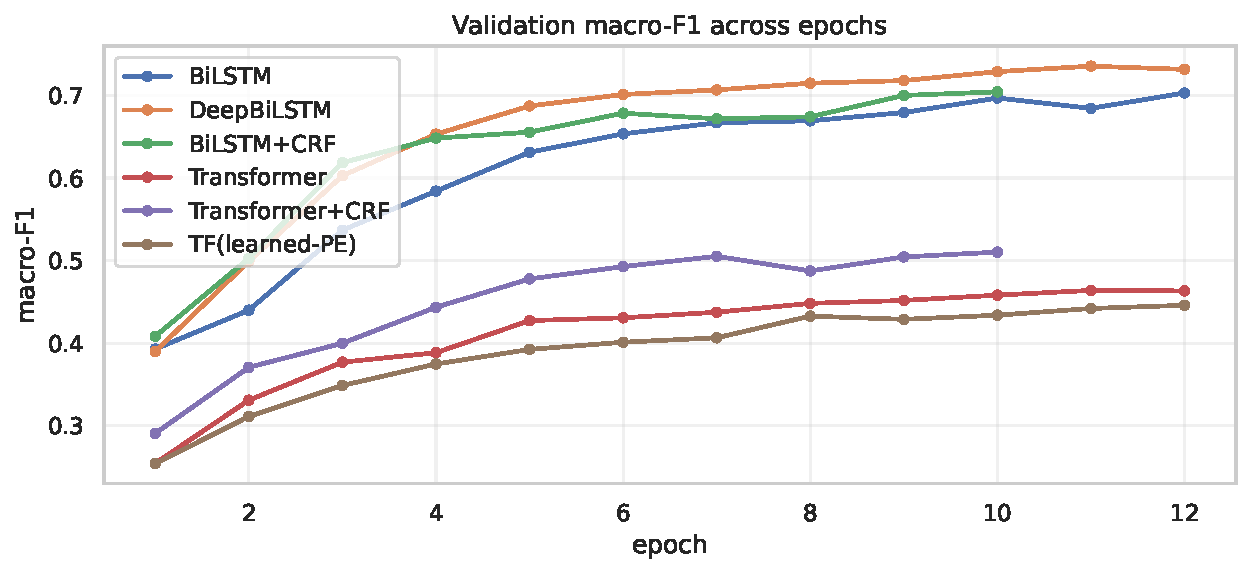
\includegraphics[width=\linewidth]{report_figures/fig_training_macroF1.pdf}
\caption{Validation macro-F1 per epoch (all six models).}
\label{fig:training}
\end{figure}

\subsection*{Validation results and best model}
Table~\ref{tab:val} compares all six models. \textbf{DeepBiLSTM} is best on
every metric (chunk-F1 0.892, macro-F1 0.736); 5-fold CV confirms stability
($0.8919\!\pm\!0.0046$). McNemar's test
\citep{McNemar1947,Dietterich1998} shows DeepBiLSTM significantly beats every
other model ($p<10^{-9}$). Figure~\ref{fig:training} shows training dynamics:
RNN models converge smoothly within 8–10 epochs while Transformers plateau lower.

Two findings emerge from the ablation (Fig.~\ref{fig:ablation}):
\begin{itemize}
    \item \textbf{Data Efficiency:} RNNs dominate Transformers by $-0.170$ chunk-F1, 
    consistent with data-efficiency results~\citep{Turc2019} at $\sim$8.9k sentences.
    
    \item \textbf{Structural Priors:} Adding the CRF helps the Transformer ($+0.107$) 
    far more than the BiLSTM ($+0.009$) — recurrence already imposes a soft 
    sequential prior that CRF makes explicit.
\end{itemize}

\begin{figure}[t]
\centering
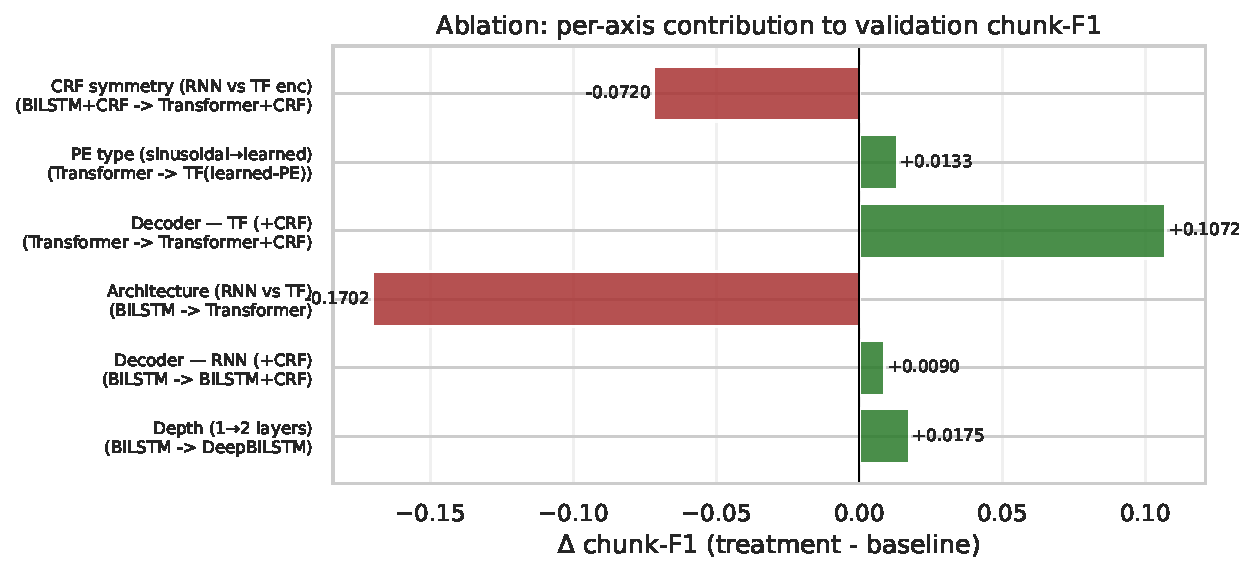
\includegraphics[width=\linewidth]{report_figures/fig_ablation_bar.pdf}
\caption{Ablation $\Delta$ChunkF1 for six single-axis comparisons.}
\label{fig:ablation}
\end{figure}

% ─────────────────────────────────────────────────────────────────────────────
\section*{Evaluate Models}
\label{sec:eval}

\subsection*{Three orthogonal metrics}
We report three metrics deliberately chosen to capture \emph{distinct}
aspects of the predictions:

\begin{itemize}
    \item \textbf{Span-level chunk-F1}~\citep{Sang2000} — the CoNLL-2000 standard:
    a span is correct iff its (type, start, end) triple matches gold exactly;
    captures \emph{chunk-correctness};
    
    \item \textbf{Cohen's $\kappa$}~\citep{Cohen1960} — chance-corrected agreement;
    captures \emph{class-imbalance robustness} (a majority-class predictor scores
    high accuracy but $\kappa\!\approx\!0$);
    
    \item \textbf{BIO sequence validity} — fraction of predicted sequences with
    no illegal transitions (e.g.\ \texttt{I-NP} after \texttt{O}); captures
    \emph{structural correctness}.
\end{itemize}

None can be derived from another: a model can have high chunk-F1 yet
low sequence validity, or high accuracy yet low~$\kappa$.

\begin{table}[t]\centering\footnotesize
\caption{Test results — DeepBiLSTM.}
\label{tab:test}
\begin{tabular}{@{}lr@{}}
\toprule
Metric (aspect) & Score \\
\midrule
\textbf{Chunk-F1} (span correctness) & \textbf{0.8979} \\
\textbf{Cohen's $\kappa$} (imbalance-robust) & \textbf{0.9267} \\
\textbf{BIO sequence validity} (structural) & \textbf{90.58\%} \\
\midrule
Token accuracy        & 94.14\% \\
Macro-F1              & 0.7278  \\
Sentence exact-match  & 44.84\% \\
\bottomrule
\end{tabular}
\end{table}

\subsection*{Test-set results}
Table~\ref{tab:test} reports DeepBiLSTM on the held-out test set across the
three metrics plus supporting diagnostics. The model achieves chunk-F1~$=0.898$,
$\kappa=0.927$ (near-perfect chance-corrected agreement), and BIO
validity~$=90.6\%$ (most sequences are structurally valid despite using a
softmax head). Sentence exact-match is 44.8\% — strict, since requiring all
$\sim$24~tokens per sentence to be simultaneously correct under 94.1\%
per-token accuracy is exponentially demanding. Per-chunk-type scores show
PP highest (0.970, closed-class prepositions are easily identified) and
ADJP lowest (0.602, low support plus frequent ADJP$\leftrightarrow$ADVP confusion).

\begin{figure}[t]
\centering
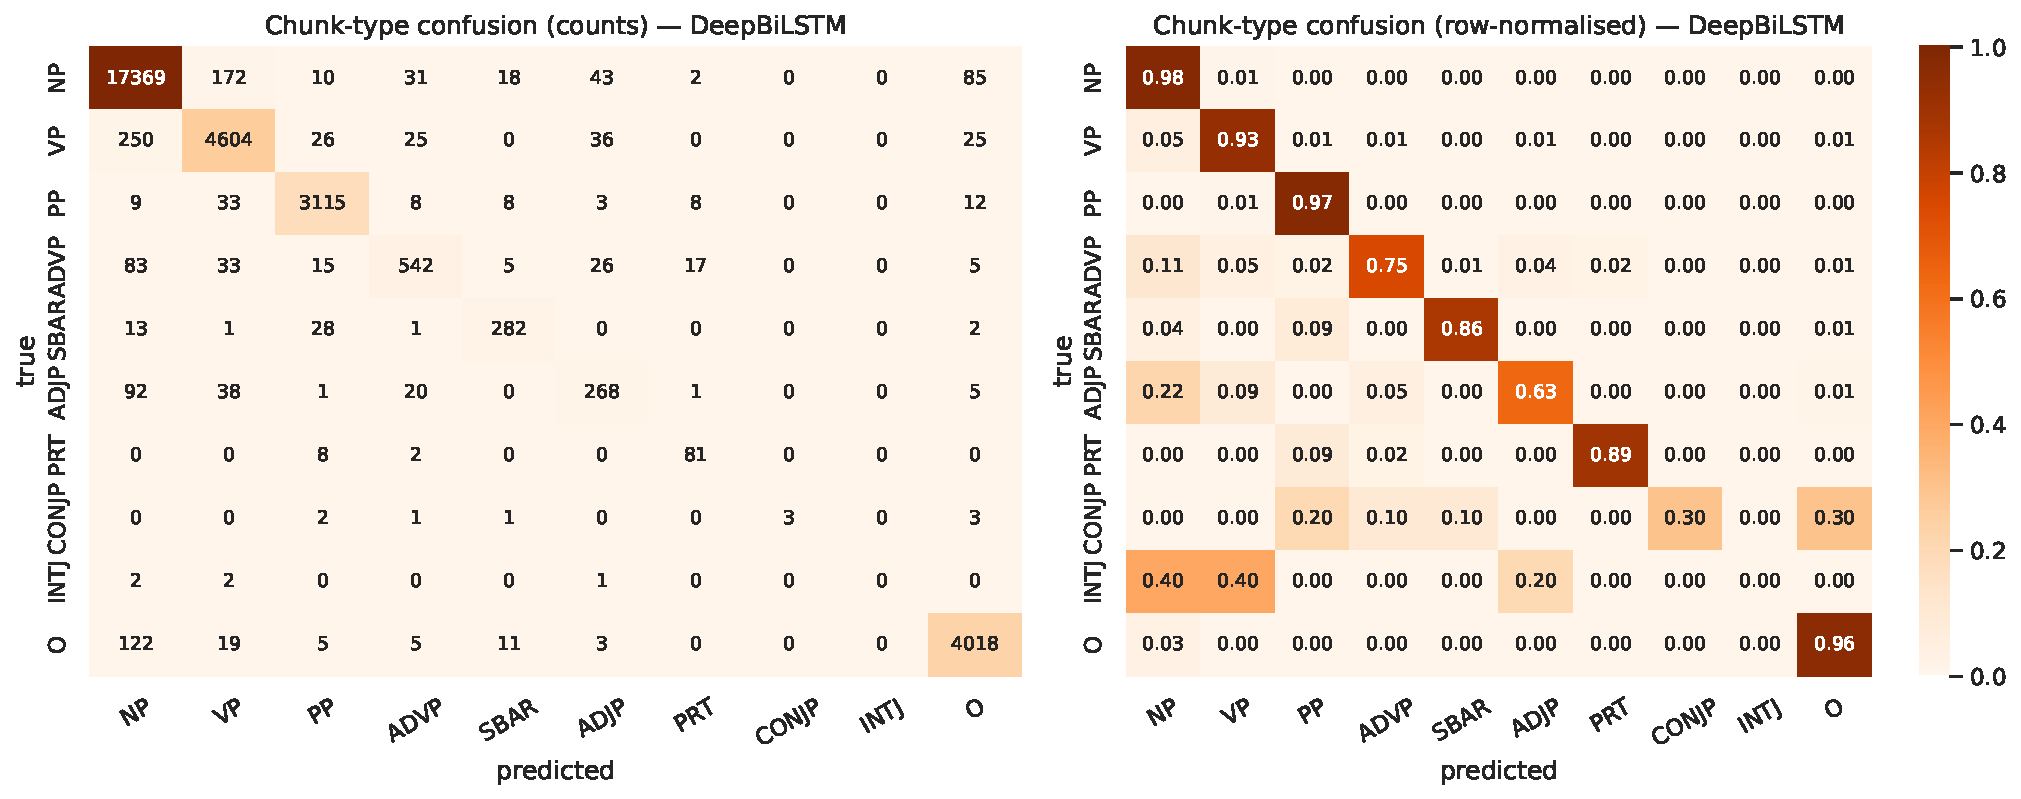
\includegraphics[width=\linewidth]{report_figures/fig_cm_chunktype.pdf}
\caption{Chunk-type confusion matrix (row-normalised).}
\label{fig:cm}
\end{figure}

\subsection*{Confusion matrix and error analysis}
Figure~\ref{fig:cm} shows the chunk-type confusion matrix (the 17$\times$17
BIO matrix is collapsed to 10 phrase families for readability). Diagonal
mass exceeds 0.85 for the four major types (NP, VP, PP, SBAR). The two
visible off-diagonal patterns are \emph{ADVP$\leftrightarrow$ADJP} confusion
(syntactically genuine ambiguity, e.g.\ \emph{``well''} as ADVP/ADJP) and
\emph{ADJP$\to$O} false negatives. Decomposing the 1{,}855 token errors:
51.3\% boundary errors (B$\leftrightarrow$I within the same family),
32.5\% type errors (different families, same prefix), 8.9\% O$\to$chunk and
7.4\% chunk$\to$O — \emph{segmentation, not classification, is the dominant
failure mode}. The CRF transition matrix (Fig.~\ref{fig:crf}) confirms valid
BIO has been learned: B-X$\to$I-X transitions are the strongest preferred
(scores $+0.85$ to $+1.09$) and O$\to$I-X transitions are penalised
($-1.20$ to $-1.21$), matching the BIO grammar.

\begin{figure}[t]
\centering
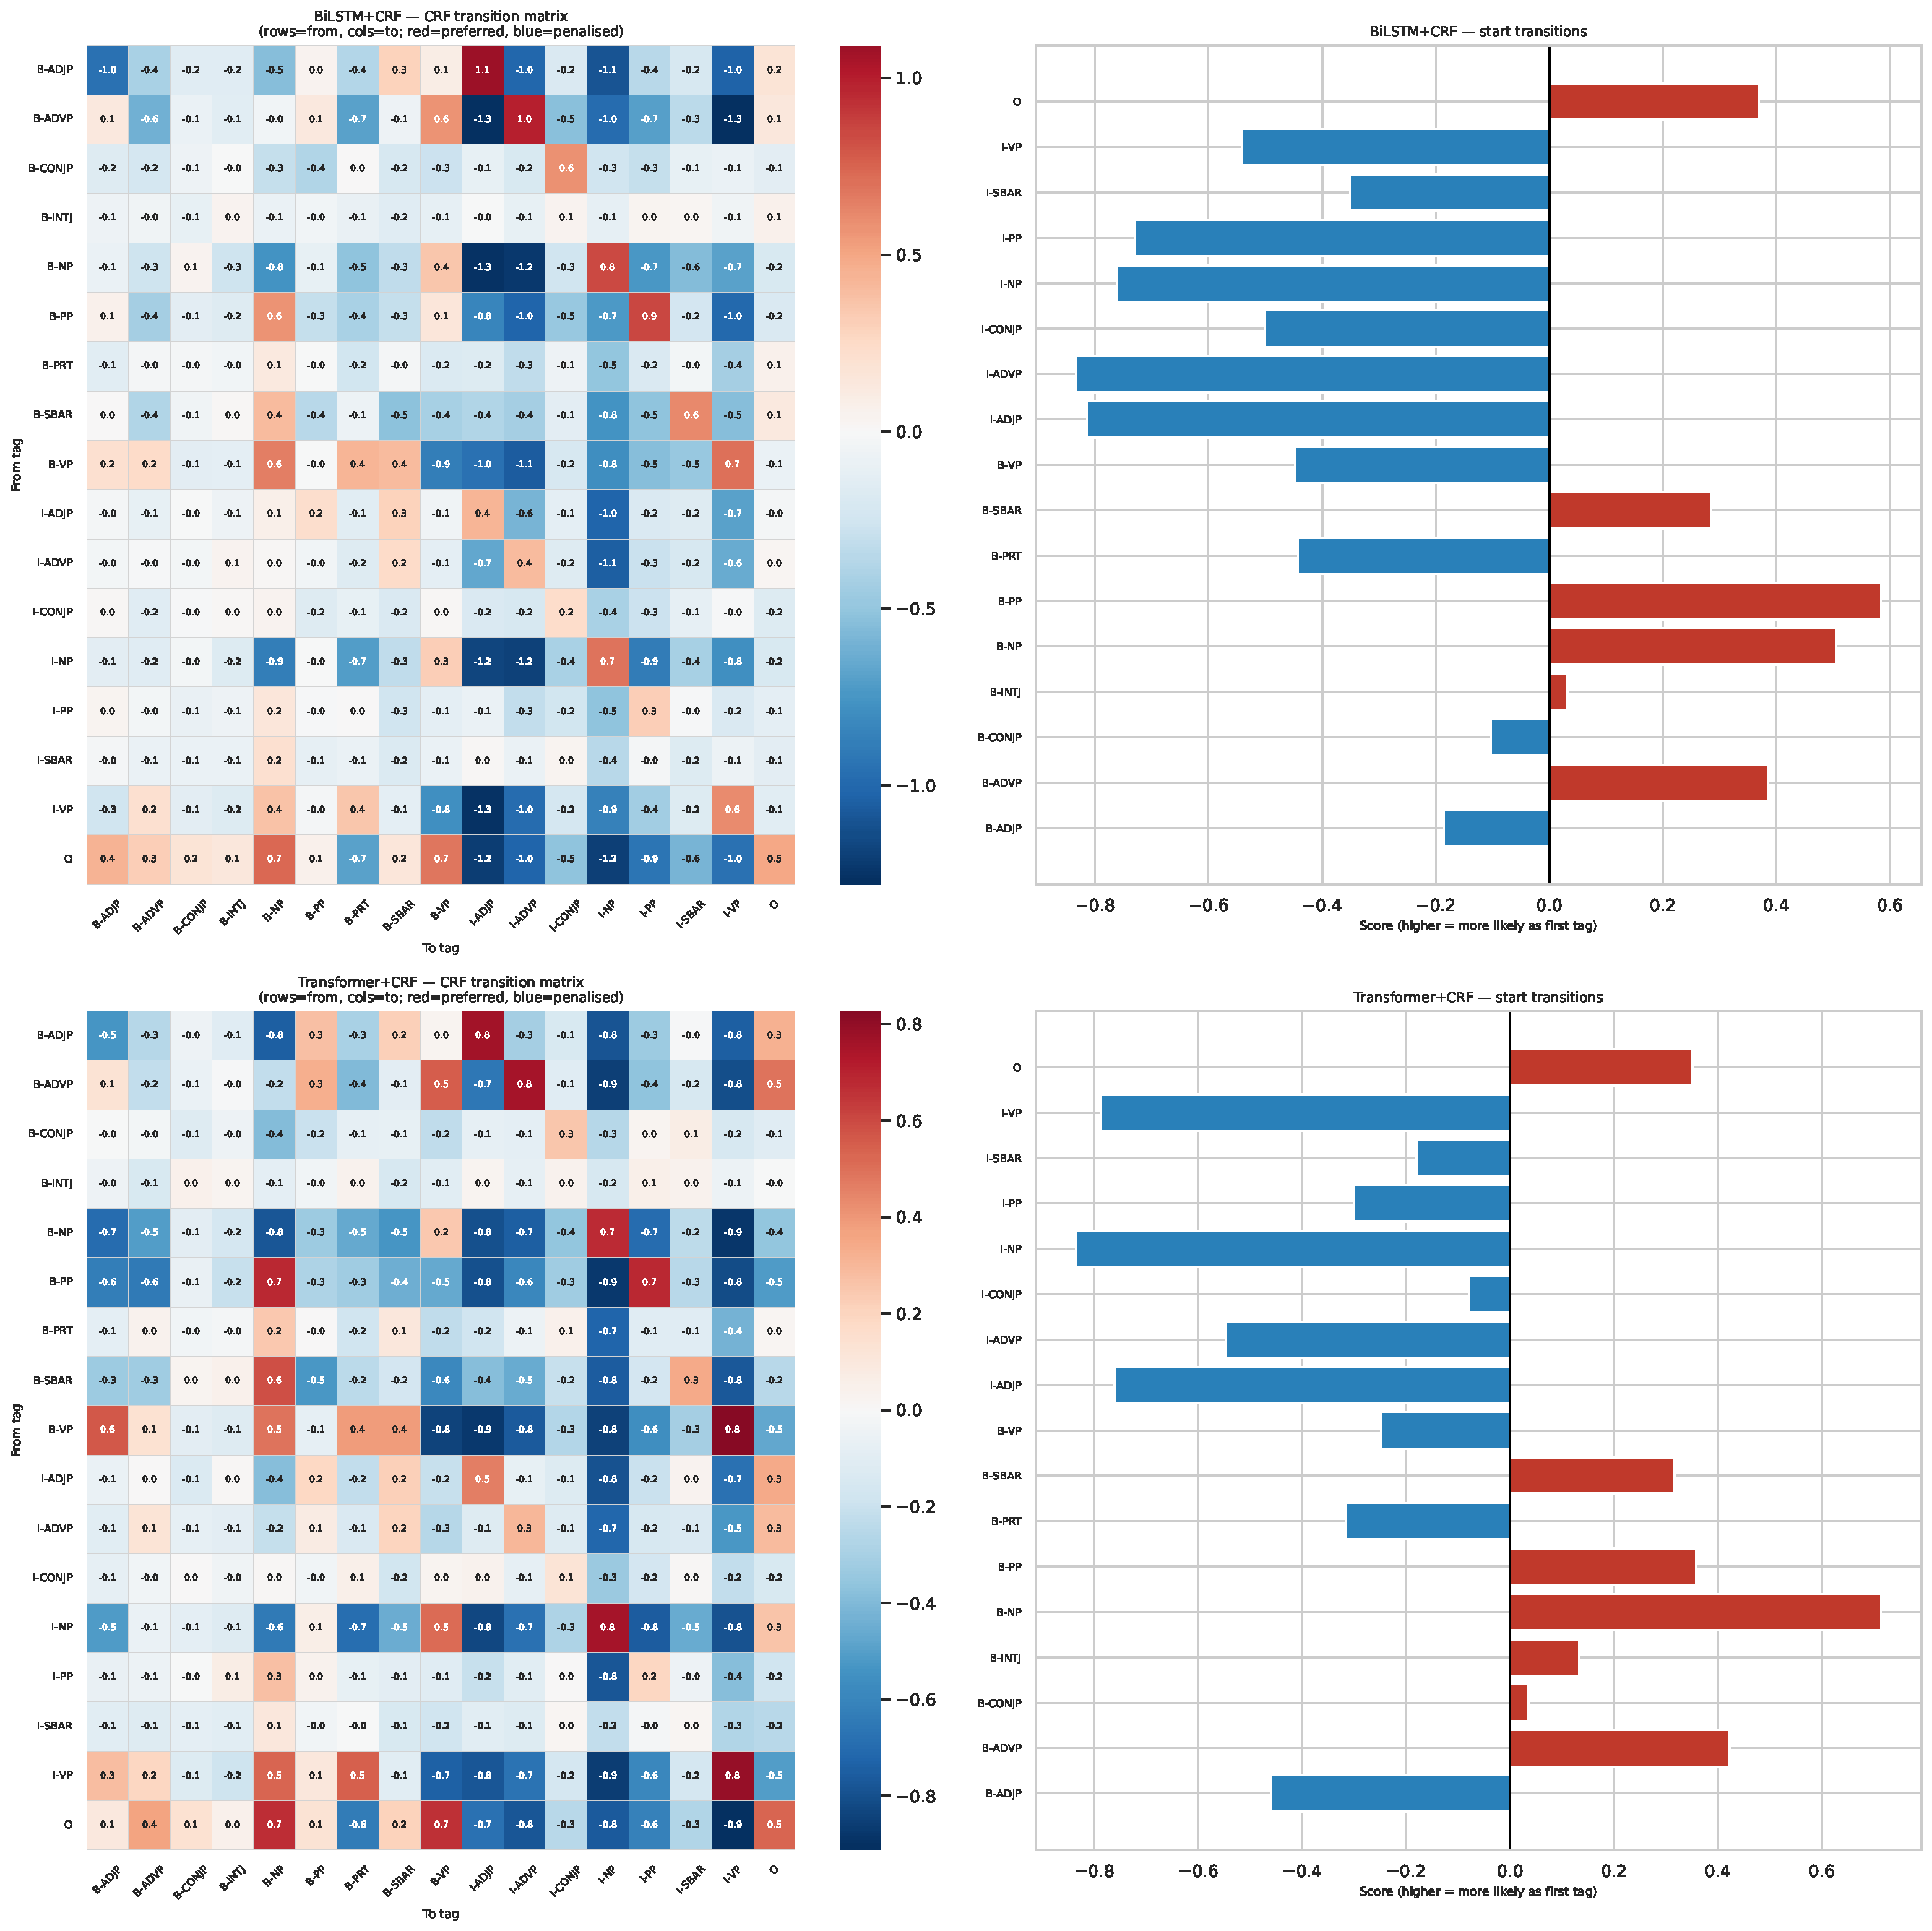
\includegraphics[width=\linewidth]{report_figures/fig_crf_transitions.pdf}
\caption{Learned CRF transition scores; red=preferred, blue=penalised.}
\label{fig:crf}
\end{figure}

% ─────────────────────────────────────────────────────────────────────────────
\section*{Conclusion}
DeepBiLSTM is the best model (chunk-F1~$=0.898$, $\kappa=0.927$,
McNemar $p<10^{-9}$). At 8.9k sentences, recurrence's inductive bias
dominates global self-attention; the CRF closes part of this gap for
Transformers. Hyperparameter search on DeepBiLSTM further raises CV
chunk-F1 to $0.902$, leaving subword/character encodings the most
promising future direction for OOV-prone phrase types.

\vspace{-2pt}
{\footnotesize\bibliographystyle{plainnat}\bibliography{refs}}

\end{document}
